\section{Background and Motivation}

\begin{frame}{Meaning Representation-to-Text Generation}
    \begin{center}
        \begin{tikzpicture}
            \node[anchor=north west] at (0,1.0)
                {\large \textbf{Input: Meaning Representation (MR)}};
            \only<1-6>{
                \node[anchor=north west] (mr) at (0,0) 
                    {$\left[\!\!\!\left[ \begin{array}{l} 
                        \textscorig{Inform} \\ 
                        \textrm{name=Aromi} \\ 
                        \textrm{eat\_type=coffee shop} \\ 
                        \textrm{area=city centre} \\ 
                    \end{array}\right]\!\!\!\right]$  };        
            }
            \only<7>{
                \node[anchor=north west] (mr) at (0,0) 
                    {$\left[\!\!\!\left[ \begin{array}{l} 
                        \textsc{Inform} \\ 
                        \textbf{\color{Red}name=Aromi} \\ 
                        \textbf{\color{Green}eat\_type=coffee shop} \\ 
                        \textbf{\color{Blue}area=city centre} \\ 
                    \end{array}\right]\!\!\!\right]$  };        
            }
            \only<2>{
                \draw[line width=0.75mm,->] (mr.south) -- (2.4,-3.5);

                \node[anchor=north west] (out) at (0,-4.0) 
                    {\large  \textbf{Output: Natural Language Utterance}};
                \node[anchor=north west,draw] (utt) at (0,-5.0) 
                    {\Large\textrm{For coffee in the city centre, try Aromi.}};
            }
            \uncover<7>{
                \draw[line width=0.75mm,->] (mr.south) -- (2.65,-3.5);

                \node[anchor=north west] (out) at (0,-4.0) 
                    {\large  \textbf{Output: Natural Language Utterance}};
                \node[anchor=north west,draw] (utt) at (0,-5.0) 
                {\Large\textrm{{\color{Green}\uline{\textbf{For coffee}}} 
                {\color{Blue}\uline{\textbf{in the city centre,}}} {\color{Red}\textbf{\uline{try Aromi.}}}}};
            }

    \uncover<3-5>{

        \node[anchor=north west,draw=mLightBrown,line width=0.5mm] (inform) at (0.43+0.05,-0.103) {\phantom{\textsc{Inform}}};
        \setbeamercolor{block title}{bg=mLightBrown,fg=white}
        \node[anchor=north west,text width=5cm,inner sep=0,outer sep=0] (da) at (5.0, -0.103) 
        {\vspace{-7.3pt}\begin{block}{Dialogue Act} 
                Goal/intent of the utterance
            \end{block}};
        \node[anchor=north west] (dafake) at (5.0,-0.103) {\phantom{\textsc{Inform}}};
        \draw[mLightBrown,thick] (inform.east) -- (dafake.west);
    }

            \uncover<4-5>{
                \node[anchor=north west,draw=Green,
                      line width=0.5mm,inner sep=0.8mm] (et) at (0.49,-1.248) 
                    {\phantom{\textrm{eat\_type}}};

                    \node[anchor=north west,line width=0.5mm,inner sep=0.8mm] 
                        (etfake1) at (-0.25,-1.248)  
                        {\phantom{\textrm{eat\_type}}};

                    \node[anchor=north west,line width=0.5mm,inner sep=0.8mm] 
                        (etfake2) at (-0.25,-3.25)  
                        {\phantom{\textrm{eat\_type}}};

                    \node[anchor=north west,line width=0.5mm,inner sep=0.8mm] 
                        (etfake3) at (0.25,-3.25)  
                        {\phantom{\textrm{eat\_type}}};

                \draw[Green,thick] (et.west) -- (etfake1.west) 
                    -- (etfake2.west) -- (etfake3.west);

                \setbeamercolor{block title}{bg=Green,fg=white}
        \node[anchor=north west,text width=4.2cm,inner sep=0,outer sep=0] (attr) at (0.0, -3.0) 
            {\begin{block}{Attributes} unordered, determines the semantics 
                of the MR\end{block}};
            }
            \uncover<5-5>{
                \node[anchor=north west,draw=VioletRed,line width=0.5mm]
                    (cc) at (1.50,-1.772) {\phantom{\textrm{city centre}}};
                \setbeamercolor{block title}{bg=VioletRed,fg=white}
                \node[anchor=north west,text width=4.0cm,inner sep=0,
                      outer sep=0] 
                    (val) at (5.0, -3.0) 
                    {\begin{block}{Attribute Values} 
                        \begin{itemize}
                            \item categorical \\ 
                            \item list-valued \\ 
                            \item free-text 
                        \end{itemize}\end{block}};

                \node[anchor=north west] (ccfake1) at (9.5, -1.772) 
                    {\phantom{\textrm{city centre}}};
                \node[anchor=north west] (ccfake2) at (9.5, -3.25) 
                    {\phantom{\textrm{city centre}}};
                \node[anchor=north west] (ccfake3) at (8.5, -3.25) 
                    {\phantom{\textrm{city centre}}};

                \draw[VioletRed,thick] (cc.east) -- (ccfake1.west) 
                    -- (ccfake2.west) -- (ccfake3.west);
            }
        \end{tikzpicture}
    \end{center}
\end{frame}

\begin{frame}{Controllable MR-to-Text Generation}
%            Surface realization order is determined by encoder, not the decoder language model.
%~\\
            
        \begin{center}
    \resizebox{0.95\textwidth}{!}{
    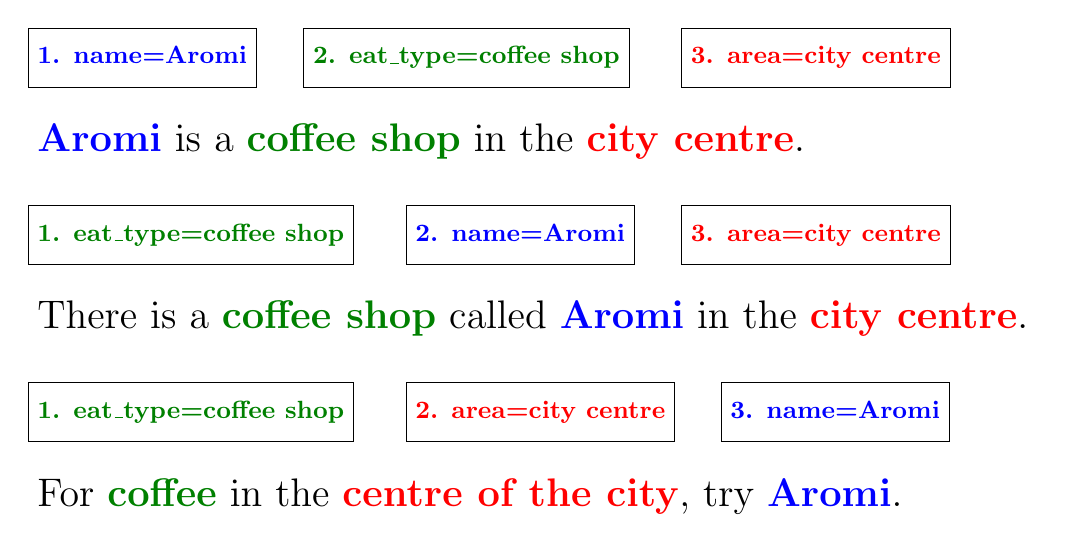
\begin{tikzpicture}
        \uncover<2->{
            \node[draw,anchor=north west,text=Blue,minimum height=0.75cm] at (0,0) {\small \textbf{1. name=Aromi\vphantom{p}}} ;
            \node[draw,anchor=north west,text=Green,minimum height=0.75cm] at (3.5,0) {\small \textbf{2. eat\_type=coffee shop}} ;
            \node[draw,anchor=north west,text=Red,minimum height=0.75cm] at (8.30,0) {\small \textbf{3. area=city centre}};
        \node[anchor=north west] at (0,-1.1) {\Large {\color{Blue}\uline{\textbf{Aromi}}} is a {\color{Green}\uline{\textbf{coffee shop}}} in the {\color{Red}\uline{\textbf{city centre}}}.};
    }
    \uncover<3->{
        \node[draw,anchor=north west,text=Green,minimum height=0.75cm] 
            at (0,-2.25) {\small \textbf{1. eat\_type=coffee shop}};
        \node[draw,anchor=north west,text=Blue,minimum height=0.75cm] 
        at (4.80,-2.25) {\small \textbf{2. name=Aromi\vphantom{p}}};
        \node[draw,anchor=north west,text=Red,minimum height=0.75cm] 
            at (8.3,-2.25) {\small \textbf{3. area=city centre}};
        \node[anchor=north west] at (0,-3.35) {\Large There is a {\color{Green}\uline{\textbf{coffee shop}}} called {\color{Blue}\uline{\textbf{Aromi}}} in the {\color{Red}\uline{\textbf{city centre}}}.} ;
    }
    \uncover<4->{
        \node[draw,anchor=north west,text=Green,minimum height=0.75cm] at (0,-4.5) {\small \textbf{1. eat\_type=coffee shop}};
        \node[draw,anchor=north west,text=Red,minimum height=0.75cm] at (4.8,-4.5) {\small \textbf{2. area=city centre}};
        \node[draw,anchor=north west,text=Blue,minimum height=0.75cm] at (8.8,-4.5) {\small \textbf{3. name=Aromi\vphantom{p}}} ;
        \node[anchor=north west] at (0,-5.6) {\Large For {\color{Green}\uline{\textbf{coffee}}} in the {\color{Red}\uline{\textbf{centre of the city}}}, try {\color{Blue}\uline{\textbf{Aromi}}}.} ;
    }



    \end{tikzpicture}
}
        \end{center}

\end{frame}





\begin{frame}{Controllable MR-to-Text Generation}


    Controllable MR-to-Text Generation will allow us to 
    \begin{itemize}
        \item implement more cognitively plausible
            discourse structuring models (e.g. Centering Theory or Accessibility Theory), 
\item more easily generate diverse outputs, and
\item confidently use neural components in NLG pipelines (Moryossef et al. (2019), Castro Ferreira et al. (2019))
    \end{itemize}
    


\end{frame}


\begin{frame}{Questions}
\begin{itemize}
\item Can you make an arbitrary sequence2sequence model controllable?
    \begin{itemize}
\item Are there differences between recurrent models or
transformers?
\item What about large pretrained models?
    \end{itemize} ~\\~\\
\item How systematic is a controllable sequence2sequence model? \\~\\
\item Can we improve systematicity with data-augmentation?~\\~\\
\end{itemize}
\end{frame}
